\section*{Problema 1}
Dado el problema de los tres cuerpos, se tienen las ecuaciones, por componentes, de movimiento
	\begin{align*}
		\ddot{x}_1 &= -\frac{Gm_2}{\abs{\vb{r}_1 - \vb{r}_2}^3} (x_1 - x_2) - \frac{Gm_3}{\abs{\vb{r}_1 - \vb{r}_3}^3} (x_1 - x_3) \\
		\ddot{y}_1 &= -\frac{Gm_2}{\abs{\vb{r}_1 - \vb{r}_2}^3} (y_1 - y_2) - \frac{Gm_3}{\abs{\vb{r}_1 - \vb{r}_3}^3} (y_1 - y_3) \\
		\ddot{x}_2 &= -\frac{Gm_2}{\abs{\vb{r}_2 - \vb{r}_1}^3} (x_2 - x_1) - \frac{Gm_3}{\abs{\vb{r}_2 - \vb{r}_3}^3} (x_2 - x_3) \\
		\ddot{y}_2 &= -\frac{Gm_2}{\abs{\vb{r}_2 - \vb{r}_1}^3} (y_2 - y_1) - \frac{Gm_3}{\abs{\vb{r}_2 - \vb{r}_3}^3} (y_2 - y_3) \\
		\ddot{x}_3 &= -\frac{Gm_2}{\abs{\vb{r}_3 - \vb{r}_1}^3} (x_3 - x_1) - \frac{Gm_3}{\abs{\vb{r}_3 - \vb{r}_2}^3} (x_3 - x_2) \\
		\ddot{y}_3 &= -\frac{Gm_2}{\abs{\vb{r}_3 - \vb{r}_1}^3} (y_3 - y_1) - \frac{Gm_3}{\abs{\vb{r}_3 - \vb{r}_2}^3} (y_3 - y_2).
	\end{align*}
Lo que nos da $12$ ecuaciones diferenciales de primer orden. Dadas las ecuaciones diferenciales, definimos las constantes y las respectivas condiciones iniciales:
\begin{description}
	\item[Masa: ] Para cada parte del sistema
	\begin{align*}
		m_1 &= 5.972\times 10^{24} \qquad (\text{Tierra}) \\
		m_3 &= 7.348\times 10^{22} \qquad (\text{Luna}) \\
		m_1 &= 1\times 10^{3} \qquad (\text{Nave}).
	\end{align*}
	\item[Condiciones Iniciales: ] Posición
	\begin{align*}
		\begin{array}{cc}
			x_1 (0) = 0, & y_1 (0) = 0, \\
			x_2 (0) = 3.844\times 10^{8}m, & y_2 (0) = 0, \\
			x_3 (0) = 6.8\times 10^{3}m, & y_3 (0) = 0.
		\end{array}
	\end{align*}
	Velocidad
	\begin{align*}
		\begin{array}{cc}
			\dot{x}_1 (0) = 0, & \dot{y}_1 (0) = 0, \\
			\dot{x}_2 (0) = 0, & \dot{y}_2 (0) = 1000m/s, \\
			\dot{x}_3 (0) = 7.5\times 10^{3} \cos{(\alpha)}m/s, & \dot{y}_3 (0) = 7.5\times 10^{3} \sin{(\alpha)}m/s.
		\end{array}
	\end{align*}
\end{description}
Con todo esto se utilizó el método Runge-Kutta de 4to orden para resolverlo. Para el primer inciso, se eliminó la masa de la luna y se graficó la orbita de la nave alrededor de la tierra.

\begin{figure}[H]
	\centering
	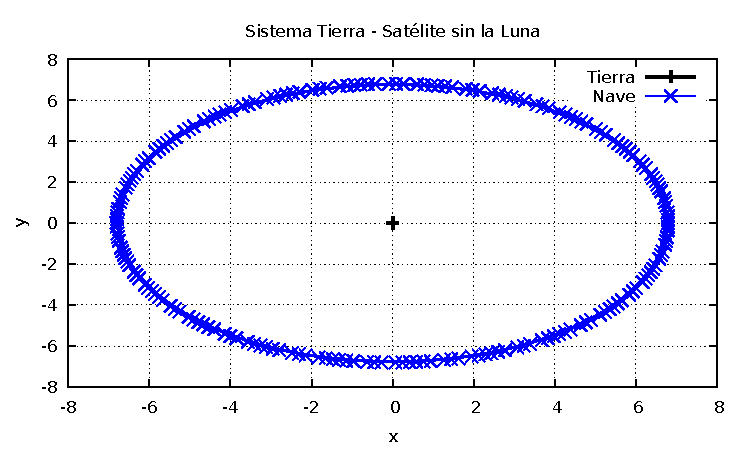
\includegraphics[scale=1]{../img/ej5-16-1.pdf}
	\caption{Gráfica de la orbita del satélite alrededor de la tierra. La gráfica no esta bajo la misma escala en ambos ejes por estética, para verla correctamente, agregar "\texttt{set size ratio -1}" en el archivo \textit{.gp}.}
\end{figure}

\begin{lstlisting}
// vie 14 oct 2022 17:25:37 CST
// ej_5-16.cpp
// Diego Sarceno (dsarceno68@gmail.com)

// Resumen

// Codificado del texto: UTF8
// Compiladores probados: g++ (Ubuntu 20.04 Linux) 9.4.0
// Instruciones de Ejecucion: no requiere nada mas
// g++ -Wall -c -o ej_5-16.o ej_5-16.cpp
// g++ -o ej_5-16.x ej_5-16.o


// Librerias
#include <iostream>
#include <cmath>
#include <iomanip>
#include <fstream>

using namespace std;

void RK4(const double *y,
		     const int n_ec,
		     const double t,
		     const double h,
		     double *y_imas1,
	             void (*derivada)( const double *, const double, double *));
void salidaSolucion(const double t, const double *y, const int N);
void spaceCraft(const double *y, const double t, double *dydt);


int main(){
  const double t0 = 0.0;
  const double h = 0.5;
  const int N = 1000000;
  const int frec_out = 5000;
  const int n_ec = 12;
  const int alpha = 0;


  // espacio de y
  double *y = new double[n_ec];
  double *y_nueva = new double[n_ec];

  // condiciones iniciales
  y[0] = 0.0;
  y[1] = 0.0;
  y[2] = 3.844e8;
  y[3] = 0.0;
  y[4] = (6.8e6)*cos(alpha);
  y[5] = (6.8e6)*sin(alpha);
  y[6] = 0.0;
  y[7] = 0.0;
  y[8] = 0.0;
  y[9] = 1000;
  y[10] = (7.5e3)*cos(M_PI_2 + alpha);
  y[11] = (7.5e3)*sin(M_PI_2 + alpha);

  // puntero a la 'derivada'
  void (*derivada)( const double *, const double, double * );
  derivada = spaceCraft;


  // incializar y_nueva
  for(int i = 0; i < n_ec; i++) y_nueva[i] = 0.0;

  double t = t0;

  // escribir las condiciones iniciales en el programa y la descripcion de las columnas de Datos
  cout << "# Columna 1: Tiempo" << endl;
  cout << "# Columna 2: Tierra-x" << endl;
  cout << "# Columna 3: Tierra-y" << endl;
  cout << "# Columna 4: Luna-x" << endl;
  cout << "# Columna 5: Luna-y" << endl;
  cout << "# Columna 6: Nave-x" << endl;
  cout << "# Columna 7: Nave-y" << endl;
  cout << "# Columna 8: Tierra-v-x" << endl;
  cout << "# Columna 9: Tierra-v-y" << endl;
  cout << "# Columna 10: Luna-v-x" << endl;
  cout << "# Columna 11: Luna-v-y" << endl;
  cout << "# Columna 12: Nave-v-x" << endl;
  cout << "# Columna 13: Nave-v-y" << endl;


  salidaSolucion(t, y, n_ec);

  for(int i = 1; i <= N; i++){
    RK4(y, n_ec, t, h, y_nueva, derivada);

    y = y_nueva;
    t += h;

    if (i % frec_out == 0){
      salidaSolucion(t, y, n_ec);
    } // END if
  } // END for
  return 0;
} // END main



void RK4(const double *y,
		     const int n_ec,
		     const double t,
		     const double h,
		     double *y_imas1,
		     void (*derivada)( const double *, const double, double *)){
  double *k0 = new double[n_ec];
  double *k1 = new double[n_ec];
  double *k2 = new double[n_ec];
  double *k3 = new double[n_ec];
  double *z  = new double[n_ec];

  (*derivada)(y, t, k0);

  for(int i=0; i<n_ec; i++)
    z[i] = y[i] + 0.5*k0[i]*h;

  (*derivada)(z, t+0.5*h, k1);

  for(int i=0; i<n_ec; i++)
    z[i] = y[i] + 0.5*k1[i]*h;

  (*derivada)(z, t+0.5*h, k2);

  for(int i=0; i<n_ec; i++)
    z[i] = y[i] + k2[i]*h;

  (*derivada)(z, t+h, k3);

  for(int i=0; i<n_ec; i++)
   y_imas1[i] = y[i] + h/6.0 * ( k0[i] + 2*k1[i] + 2*k2[i] + k3[i] );

  delete[] k0;
  delete[] k1;
  delete[] k2;
  delete[] k3;
  delete[] z;
}





void salidaSolucion(const double t, const double *y, const int N){
  cout << fixed << setprecision(3) << t;

  for( int i=0; i<N; i++ )
    cout << scientific << setprecision(9) << "\t" << y[i];

  cout << endl;
}




void spaceCraft(const double *y, const double t, double *dydt){
  const double m1 = 5.972e24; //masa de la tierra
  const double m2 = 7.348e22; //masa de la luna
	//const double m2 = 0.0; // masa de la luna, prueba ej 1
  const double m3 = 1000; //masa de la nave
  const double G  = 6.66e-11; // Constante de gravitacion universal

  // distancias
  const double r21_3 = pow( pow(y[2]-y[0],2) + pow(y[3]-y[1],2), 1.5 );
  const double r31_3 = pow( pow(y[4]-y[0],2) + pow(y[5]-y[1],2), 1.5 );
  const double r32_3 = pow( pow(y[4]-y[2],2) + pow(y[5]-y[3],2), 1.5 );
	ofstream truefalse;

	truefalse.open("truefalse", ios::out);
	if(r32_3 <= 3.8e6){
		truefalse << r32_3 << endl;
	} // END if



  dydt[0]  = y[6];
  dydt[1]  = y[7];
  dydt[2]  = y[8];
  dydt[3]  = y[9];
  dydt[4]  = y[10];
  dydt[5]  = y[11];
  dydt[6]  = -G*m2*( y[0]-y[2] ) / r21_3 - G*m3*( y[0]-y[4] ) / r31_3;
  dydt[7]  = -G*m2*( y[1]-y[3] ) / r21_3 - G*m3*( y[1]-y[5] ) / r31_3;
  dydt[8]  = -G*m1*( y[2]-y[0] ) / r21_3 - G*m3*( y[2]-y[4] ) / r32_3;
  dydt[9]  = -G*m1*( y[3]-y[1] ) / r21_3 - G*m3*( y[3]-y[5] ) / r32_3;
  dydt[10] = -G*m1*( y[4]-y[0] ) / r31_3 - G*m2*( y[4]-y[2] ) / r32_3;
  dydt[11] = -G*m1*( y[5]-y[1] ) / r31_3 - G*m2*( y[5]-y[3] ) / r32_3;
} // END spaceCraft

\end{lstlisting}




\section*{Problema 2}
Para este problema únicamente se jugó con las condiciones iniciales, variando parámetros como $\alpha$ y $v_o$. Se llegó a las siguientes condiciones iniciales para que la nave pasara por la luna.

\begin{description}
	\item[Posición: ] $x_3 (0) = 6.8\times 10^6 m$ y $y_3 (0) = 0.$ Es decir un $\alpha = 0$.
	\item[Velocidad: ] $\dot{x} _3 (0) = 2.5\times 10^4 m/s$ y $\dot{y} _3 (0) = 0m/s$. 
\end{description}
Dejando la siguiente gráfica
\begin{figure}[H]
	\centering
	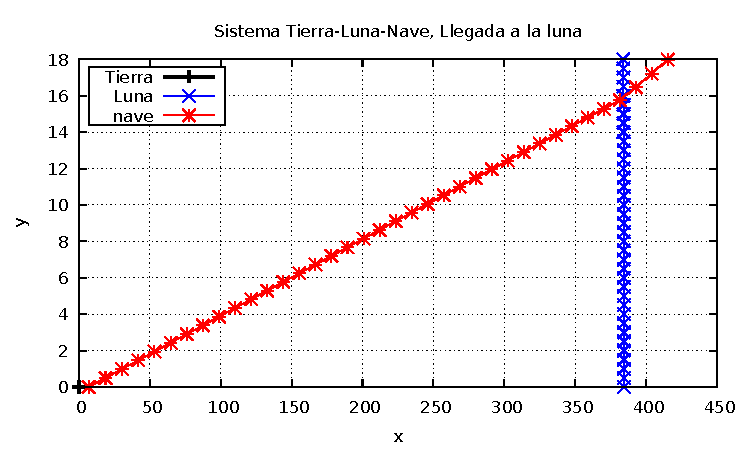
\includegraphics[scale=0.8]{../img/ej5-17.pdf}
	\caption{Es claro que la nave pasa lo suficientemente cerca de la luna.}
	\label{ej5-17}
\end{figure}











\section*{Problema 3}
Bajo la misma idea del ejercicio anterior, se econtraron las siguientes condiciones iniciales.
\begin{description}
	\item[Posición: ] $x_3 (0) = 6.8\times 10^6 \cos{(36.869^o)} m$ y $y_3 (0) = 6.8\times 10^6 \sin{(36.869^o)} m.$ Es decir un $\alpha = 36.869^o$.
	\item[Velocidad: ] $\dot{x} _3 (0) = 7728 m/s$ y $\dot{y} _3 (0) = 7420m/s$, se utilizó otro ángulo por pura prueba y error. 
\end{description}
Dejando la siguiente gráfica
\begin{figure}[H]
	\centering
	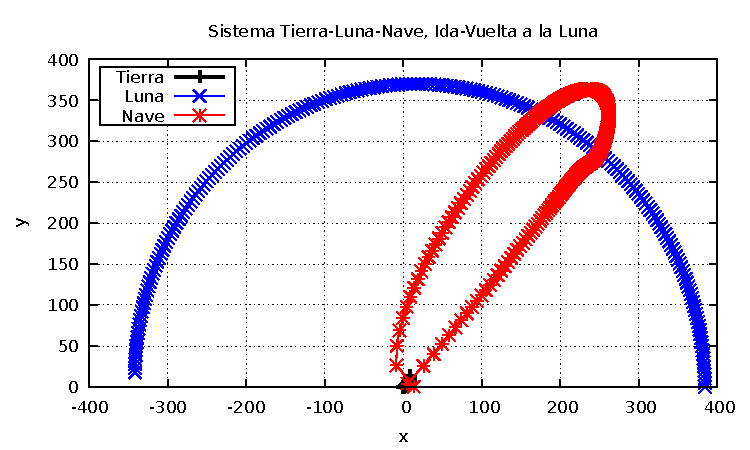
\includegraphics[scale=0.8]{../img/ej5-18.pdf}
	\caption{Es claro que la nave pasa lo suficientemente cerca de la luna como para forzar un retorno en su trayectoria.}
	\label{ej5-17}
\end{figure}













%%%%%%%